\subsection{OTFS-IM Transmitter Design}

This section describes how the OTFS-IM transmitter constructs the delay-Doppler input grid used by the common OTFS modulation block. Compared with the baseline OTFS transmitter in Chapter 3, the new operation is the block-wise mapping from input bits to activation patterns and active QAM symbols. After the OTFS-IM grid is formed, the ISFFT and Heisenberg transform are reused without structural modification.

\subsubsection{Overview of the OTFS-IM Transmitter Processing Chain}

The transmitter starts from a binary vector of length \(\lambda\), where
\begin{equation}
    \lambda = g(b_1+b_2).
\end{equation}
This vector is processed block by block. In each block, the first \(b_1\) bits select the activation pattern, while the following \(b_2\) bits are mapped to QAM symbols. Only the selected active positions are filled with QAM symbols; all other positions remain zero.

Figure~\ref{fig:otfs_im_transmitter_flow} summarizes the implemented transmitter processing flow. The purpose of the figure is to show the internal OTFS-IM mapping stage before the standard OTFS modulation block is applied.

\begin{figure}[H]
    \centering
    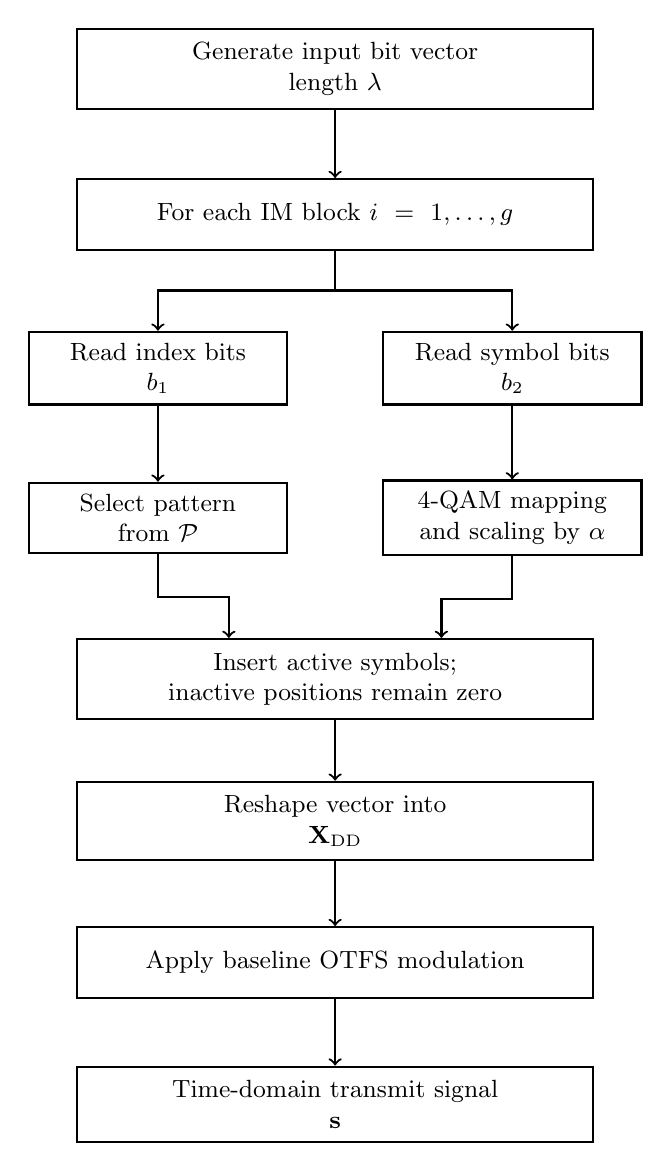
\begin{tikzpicture}[
        block/.style={
            rectangle,
            draw,
            thick,
            align=center,
            text width=6.2cm,
            minimum height=0.9cm,
            font=\small,
            inner sep=5pt
        },
        smallblock/.style={
            rectangle,
            draw,
            thick,
            align=center,
            text width=3.0cm,
            minimum height=0.85cm,
            font=\small,
            inner sep=4pt
        },
        arrow/.style={->, thick}
    ]

        \node[block] (bits) at (0,0) {Generate input bit vector\\length \(\lambda\)};
        \node[block] (loop) at (0,-1.85) {For each IM block \(i=1,\ldots,g\)};
        \node[smallblock] (idx) at (-2.25,-3.8) {Read index bits\\\(b_1\)};
        \node[smallblock] (sym) at (2.25,-3.8) {Read symbol bits\\\(b_2\)};
        \node[smallblock] (pat) at (-2.25,-5.7) {Select pattern\\from \(\mathcal{P}\)};
        \node[smallblock] (qam) at (2.25,-5.7) {4-QAM mapping\\and scaling by \(\alpha\)};
        \node[block] (insert) at (0,-7.75) {Insert active symbols;\\inactive positions remain zero};
        \node[block] (reshape) at (0,-9.55) {Reshape vector into\\\(\mathbf{X}_{\mathrm{DD}}\)};
        \node[block] (otfs) at (0,-11.35) {Apply baseline OTFS modulation};
        \node[block] (tx) at (0,-13.15) {Time-domain transmit signal\\\(\mathbf{s}\)};

        \draw[arrow] (bits.south) -- (loop.north);
        \draw[arrow] (loop.south) -- ++(0,-0.5) -| (idx.north);
        \draw[arrow] (loop.south) -- ++(0,-0.5) -| (sym.north);
        \draw[arrow] (idx.south) -- (pat.north);
        \draw[arrow] (sym.south) -- (qam.north);
        \draw[arrow] (pat.south) -- ++(0,-0.55) -| ([xshift=-1.35cm]insert.north);
        \draw[arrow] (qam.south) -- ++(0,-0.55) -| ([xshift=1.35cm]insert.north);
        \draw[arrow] (insert.south) -- (reshape.north);
        \draw[arrow] (reshape.south) -- (otfs.north);
        \draw[arrow] (otfs.south) -- (tx.north);

    \end{tikzpicture}
    \caption{OTFS-IM transmitter processing flow}
    \label{fig:otfs_im_transmitter_flow}
\end{figure}

This flow also reflects the separation between the proposed OTFS-IM mapping and the baseline OTFS modulation. The index-modulation part determines the sparse delay-Doppler grid, while the modulation part converts this grid into the transmitted time-domain waveform.

\subsubsection{Index and Symbol Bit Mapping}

For the \(i\)-th IM block, the transmitter reads \(b_1\) index bits and converts them into a decimal value. Let this value be denoted by \(q_i\). The implemented mapping then converts \(q_i\) into a Gray index:
\begin{equation}
    m_i
    =
    q_i
    \oplus
    \left\lfloor
    \frac{q_i}{2}
    \right\rfloor ,
    \label{eq:tx_gray_index}
\end{equation}
where \(\oplus\) denotes bitwise exclusive-or.
The selected activation pattern is then obtained from the pattern table:
\begin{equation}
    \mathbf{p}_{m_i}
    =
    \mathcal{P}[m_i].
    \label{eq:tx_pattern_selection}
\end{equation}
The entries of \(\mathbf{p}_{m_i}\) are local active positions inside the current IM block.

The next \(b_2\) bits are used to generate the active QAM symbols. Since
\begin{equation}
    b_2 = k\log_2(M_{\mathrm{mod}}),
\end{equation}
these bits form exactly \(k\) modulation symbols. In this thesis, \(M_{\mathrm{mod}}=4\), so each active position carries one 4-QAM symbol. The generated QAM symbols are multiplied by the normalization factor
\begin{equation}
    \alpha = \sqrt{\frac{n}{k}},
\end{equation}
which preserves the average block energy when only \(k\) out of \(n\) positions are active.

After one IM block is processed, the bit-reading position is advanced by \(b_1+b_2\) bits. This ensures that the input vector is consumed sequentially and that each block carries one index label and \(k\) active QAM symbols.

\subsubsection{Illustrative Block-Mapping Example}

To clarify the mapping process, consider the representative configuration \((n,k)=(4,3)\) with 4-QAM. In this case, there are
\begin{equation}
    \binom{4}{3}=4
\end{equation}
valid constant-weight activation patterns. Therefore,
\begin{equation}
    b_1=\left\lfloor \log_2 4 \right\rfloor=2,
    \qquad
    b_2=3\log_2(4)=6.
\end{equation}
Each IM block carries \(b_1+b_2=8\) information bits. The first two bits select one activation pattern, and the next six bits generate three 4-QAM symbols.

Suppose that the selected activation pattern is
\begin{equation}
    \mathbf{p}_{m_i}=[1,2,4].
\end{equation}
Then the first, second, and fourth local positions of the IM block are active, while the third local position is inactive. If the three scaled QAM symbols for this block are denoted by \(\alpha s_{i,1}\), \(\alpha s_{i,2}\), and \(\alpha s_{i,3}\), the local block vector becomes
\begin{equation}
    \mathbf{x}_{i}
    =
    \left[
    \alpha s_{i,1},
    \alpha s_{i,2},
    0,
    \alpha s_{i,3}
    \right]^{T}.
    \label{eq:otfs_im_local_block_example}
\end{equation}
This example shows the two-layer information structure of OTFS-IM. The nonzero symbol values carry QAM information, while the zero position carries index information because its location is part of the selected activation pattern.

For the next IM block, the same procedure is repeated on the next group of \(n\) delay-Doppler positions. Thus, the full OTFS-IM frame is not one arbitrary sparse vector. It is a structured sparse vector formed by concatenating \(g\) local IM blocks, each of which has exactly \(k\) active positions. This structure is what makes block-wise MAP detection possible at the receiver.

\subsubsection{Delay-Doppler Grid Construction}

The vectorized OTFS-IM delay-Doppler frame is denoted by \(\mathbf{x}_{\mathrm{vec}}\). It has length \(NM\) and is initialized as an all-zero vector:
\begin{equation}
    \mathbf{x}_{\mathrm{vec}} \in \mathbb{C}^{NM \times 1}.
\end{equation}
For the \(i\)-th IM block, the local positions are
\begin{equation}
    \mathcal{B}_i
    =
    \{(i-1)n+1,\ldots,in\}.
\end{equation}
If the selected local active pattern is \(\mathbf{p}_{m_i}\), then the global active positions are
\begin{equation}
    (i-1)n + \mathbf{p}_{m_i}.
    \label{eq:tx_global_active_positions}
\end{equation}
Only these positions are filled with the scaled QAM symbols. In compact form, the assignment can be written as
\begin{equation}
    \mathbf{x}_{\mathrm{vec}}\big((i-1)n+\mathbf{p}_{m_i}\big)
    =
    \alpha \mathbf{s}_i,
    \label{eq:tx_xvec_assignment}
\end{equation}
where \(\mathbf{s}_i\) contains the \(k\) QAM symbols of the \(i\)-th IM block.

All inactive positions remain zero by construction. This choice is simple but important: zeros are not missing symbols; they are intentional inactive resource elements that carry index information through their locations.

After all \(g\) IM blocks have been processed, the vector \(\mathbf{x}_{\mathrm{vec}}\) is reshaped into the \(N \times M\) delay-Doppler grid:
\begin{equation}
    \mathbf{X}_{\mathrm{DD}}
    =
    \mathrm{reshape}
    \left(
    \mathbf{x}_{\mathrm{vec}}, N, M
    \right).
    \label{eq:tx_xdd_reshape}
\end{equation}
This grid is the OTFS-IM counterpart of the full QAM delay-Doppler grid used in the baseline OTFS transmitter. The difference is that \(\mathbf{X}_{\mathrm{DD}}\) now contains both active QAM entries and inactive zero entries.

\subsubsection{Connection to the Baseline OTFS Modulation Block}

Once the OTFS-IM delay-Doppler grid has been constructed, the remaining modulation process is identical to the baseline OTFS transmitter. The OTFS-IM transmit signal can be written compactly as
\begin{equation}
    \mathbf{s}_{\mathrm{IM}}
    =
    \mathcal{M}_{\mathrm{OTFS}}
    \left\{
    \mathbf{X}_{\mathrm{DD}}
    \right\},
    \label{eq:otfs_im_common_modulation}
\end{equation}
where \(\mathcal{M}_{\mathrm{OTFS}}\{\cdot\}\) denotes the common OTFS modulation operation. The delay-Doppler grid is first transformed into the time-frequency domain using the ISFFT operation, and the time-domain transmit signal is then obtained through the discrete Heisenberg transform. Therefore, the transmitter design in this chapter does not redefine the OTFS modulation theory from Chapter 3. Instead, it changes the content of the delay-Doppler input grid before the common OTFS modulation block is applied.

This modular structure is useful for a fair comparison. Baseline OTFS and OTFS-IM share the same frame size, channel model, OTFS modulation and demodulation operations, and detector foundation. The main difference is the delay-Doppler grid construction. Consequently, the simulation results in Chapter 5 can attribute performance differences mainly to the use of index modulation and activation-pattern design rather than to a different physical-layer waveform implementation.
